\documentclass[border=4pt]{standalone}
\usepackage{amsmath,amssymb,tikz}
\usetikzlibrary{arrows.meta,calc,matrix,positioning}
\definecolor{figB}{RGB}{31,90,166}\definecolor{figR}{RGB}{176,48,48}\definecolor{figG}{RGB}{46,125,50}\definecolor{figO}{RGB}{214,120,20}
\begin{document}
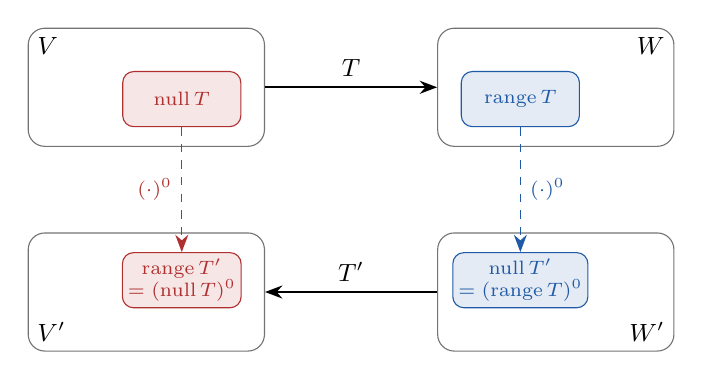
\begin{tikzpicture}[>={Stealth[length=2.2mm]},
  space/.style={draw=black!55,rounded corners=6pt,minimum width=3.0cm,minimum height=1.5cm},
  sub/.style={rounded corners=4pt,minimum width=1.5cm,minimum height=0.7cm,font=\scriptsize,inner sep=2pt}]
\node[space] (V) at (0,0) {}; \node[font=\small,anchor=north west] at (V.north west) {$V$};
\node[space] (W) at (5.2,0) {}; \node[font=\small,anchor=north east] at (W.north east) {$W$};
\node[space] (Vd) at (0,-2.6) {}; \node[font=\small,anchor=south west] at (Vd.south west) {$V'$};
\node[space] (Wd) at (5.2,-2.6) {}; \node[font=\small,anchor=south east] at (Wd.south east) {$W'$};
\node[sub,draw=figR,fill=figR!12,text=figR] (nT) at (0.45,-0.15) {$\operatorname{null}T$};
\node[sub,draw=figB,fill=figB!12,text=figB] (rT) at (4.75,-0.15) {$\operatorname{range}T$};
\node[sub,draw=figR,fill=figR!12,text=figR,align=center] (rTd) at (0.45,-2.45) {$\operatorname{range}T'$\\$=(\operatorname{null}T)^0$};
\node[sub,draw=figB,fill=figB!12,text=figB,align=center] (nTd) at (4.75,-2.45) {$\operatorname{null}T'$\\$=(\operatorname{range}T)^0$};
\draw[->,thick] (V.east)--(W.west) node[midway,above,font=\small]{$T$};
\draw[->,thick] (Wd.west)--(Vd.east) node[midway,above,font=\small]{$T'$};
\draw[->,figR,dashed] (nT.south)--(rTd.north) node[midway,left,font=\scriptsize]{$(\cdot)^0$};
\draw[->,figB,dashed] (rT.south)--(nTd.north) node[midway,right,font=\scriptsize]{$(\cdot)^0$};
\end{tikzpicture}
\end{document}
